% 图 6.25 铁晶须表面畴图样随外场演化（五个面板，右侧磁场增强方向）
\documentclass[tikz,border=5pt]{standalone}
\usetikzlibrary{arrows.meta}
\usepackage{amsmath}
\usepackage{bm}
\usepackage{fontspec}
\setmainfont{Times New Roman}
\begin{document}
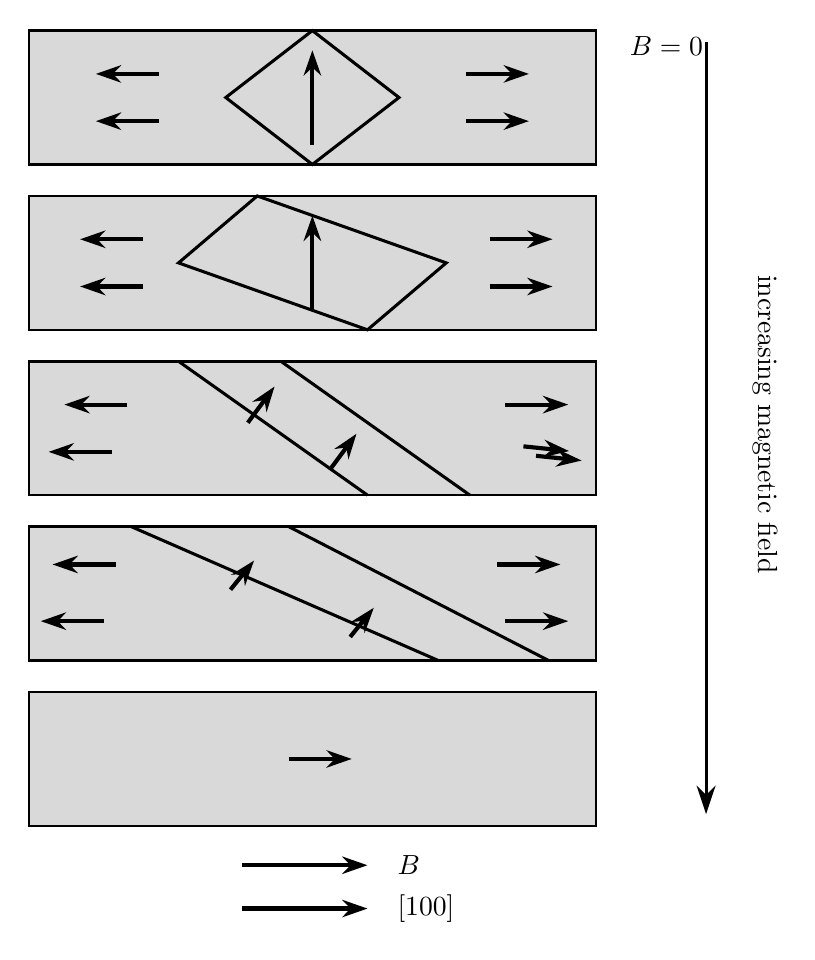
\begin{tikzpicture}[line width=0.8pt,>=Stealth,
  mag/.style={->,line width=1.5pt,>={Stealth[length=3.2mm,width=2.2mm]}},
  panel/.style={fill=gray!30,line width=0.9pt},
  wall/.style={line width=1.1pt}]
% ---- panel 1 : B = 0 ----
\draw[panel] (0,8.4) rectangle (7.2,10.1);
\draw[wall] (3.6,10.1) -- (2.5,9.25) -- (3.6,8.4) -- (4.7,9.25) -- cycle;
\draw[mag] (1.65,9.55) -- (0.85,9.55);
\draw[mag] (1.65,8.95) -- (0.85,8.95);
\draw[mag] (5.55,9.55) -- (6.35,9.55);
\draw[mag] (5.55,8.95) -- (6.35,8.95);
\draw[mag] (3.6,8.65) -- (3.6,9.85);
% ---- panel 2 ----
\begin{scope}[shift={(0,-2.1)}]
  \draw[panel] (0,8.4) rectangle (7.2,10.1);
  \draw[wall] (2.9,10.1) -- (1.9,9.25) -- (4.3,8.4) -- (5.3,9.25) -- cycle;
  \draw[mag] (1.45,9.55) -- (0.65,9.55);
  \draw[mag] (1.45,8.95) -- (0.65,8.95);
  \draw[mag] (5.85,9.55) -- (6.65,9.55);
  \draw[mag] (5.85,8.95) -- (6.65,8.95);
  \draw[mag] (3.6,8.65) -- (3.6,9.85);
\end{scope}
% ---- panel 3 ----
\begin{scope}[shift={(0,-4.2)}]
  \draw[panel] (0,8.4) rectangle (7.2,10.1);
  \draw[wall] (1.9,10.1) -- (4.3,8.4);
  \draw[wall] (3.2,10.1) -- (5.6,8.4);
  \draw[mag] (2.78,9.32) -- (3.12,9.78);
  \draw[mag] (3.82,8.72) -- (4.16,9.18);
  \draw[mag] (1.25,9.55) -- (0.45,9.55);
  \draw[mag] (1.05,8.95) -- (0.25,8.95);
  \draw[mag] (6.05,9.55) -- (6.85,9.55);
  \draw[mag] (6.28,9.02) -- (6.86,8.96);
  \draw[mag] (6.44,8.9)  -- (7.02,8.84);
\end{scope}
% ---- panel 4 ----
\begin{scope}[shift={(0,-6.3)}]
  \draw[panel] (0,8.4) rectangle (7.2,10.1);
  \draw[wall] (1.3,10.1) -- (5.2,8.4);
  \draw[wall] (3.3,10.1) -- (6.6,8.4);
  \draw[mag] (2.56,9.3) -- (2.86,9.67);
  \draw[mag] (4.08,8.7)  -- (4.38,9.07);
  \draw[mag] (1.1,9.62) -- (0.3,9.62);
  \draw[mag] (0.95,8.9) -- (0.15,8.9);
  \draw[mag] (5.95,9.62) -- (6.75,9.62);
  \draw[mag] (6.05,8.9) -- (6.85,8.9);
\end{scope}
% ---- panel 5 : saturated single domain ----
\begin{scope}[shift={(0,-8.4)}]
  \draw[panel] (0,8.4) rectangle (7.2,10.1);
  \draw[mag] (3.3,9.25) -- (4.1,9.25);
\end{scope}
% ---- B = 0 label, field-direction arrow and text ----
\node[anchor=west] at (7.5,9.9) {$B=0$};
\draw[->,line width=1.1pt,>={Stealth[length=3.6mm,width=2.4mm]}] (8.6,9.95) -- (8.6,0.15);
\node[rotate=-90] at (9.35,5.1) {increasing magnetic field};
% ---- B and [100] arrows at bottom ----
\draw[mag] (2.7,-0.5) -- (4.3,-0.5);
\node[anchor=west] at (4.55,-0.5) {$B$};
\draw[mag] (2.7,-1.05) -- (4.3,-1.05);
\node[anchor=west] at (4.55,-1.05) {$[100]$};
\end{tikzpicture}
\end{document}
